\documentclass{beamer}

% Style:
\usepackage{fontspec}
\setsansfont{Candara}
\usetheme{Rochester}
\definecolor{primarycolor}{RGB}{15,20,40}
\usecolortheme[named=primarycolor]{structure}
\setbeamercolor{normal text}{fg=primarycolor}
\setbeamertemplate{caption}{\raggedright\insertcaption\par}
\setbeamertemplate{bibliography item}[text]

% For tables:
\usepackage{colortbl}
\definecolor{bestcol}{RGB}{99, 255, 105}
\definecolor{secondbestcol}{RGB}{250, 255, 99}
\definecolor{worstcol}{RGB}{255, 141, 99}
\usepackage{arydshln}

\usepackage{ulem}

\title{\textsc{\bfseries Transfer Learning with\\Vision Transformers}}
\author{\textbf{Vincent} Tonkes}
\institute{\textbf{University} of Groningen}
\date{}

% Also makes it bold and small caps
\newcommand{\createtitle}[1]{\frametitle{\textsc{\bfseries#1}}}

% Make \cite commands tiny
\newcommand{\tinycite}[1]{{\tiny \cite{#1}}}

\begin{document}

%-------------------------------------------------------------------------------
% Leaves them out on slide two and highlights them on slide 3
{
\setbeamercolor*{frametitle}{bg=white}
\frame{
\titlepage
{\tiny Supervised by:}\\\small\textbf{Matthia} Sabatelli\tiny, PhD
}
}

%-------------------------------------------------------------------------------

%-------------------------------------------------------------------------------
\newcommand{\toexplain}[1]{
    \textcolor<2>{white}{\textcolor<3>{red}{#1}}
}
\begin{frame}
\createtitle{Research Question}
\begin{center}
\textbf{\large ``\textit{To what extent (and in what manners) does utilizing \toexplain{Transfer Learning} allow \toexplain{Vision Transformers} to perform on par with \toexplain{Convolutional Neural Networks} on common \toexplain{art classification problems}, when compute resources are limited to a single \toexplain{GPU}?}''}
\end{center}
\end{frame}
%-------------------------------------------------------------------------------

%-------------------------------------------------------------------------------
% IT HURTS, but I have to remove this because its too long already D-':
%\begin{frame}
%\createtitle{Transfer Learning}

%\begin{columns}
%\pause
%\column{0.5\textwidth}
%{\large Learning = \textbf{Machine} Learning:}
%\pause
%\begin{itemize}
%\item Data that `summarizes' all previous learning experiences;
%\pause
%\item Way of updating that data with new experiences;
%\pause
%\item Way of making decisions based on that data.
%\pause
%\end{itemize}

%\column{0.5\textwidth}
%But what about Artificial Neural Networks?
%\begin{figure}
%\input{img/ann.pdf_tex}
%\end{figure}

%\end{columns}
%\end{frame}
%-------------------------------------------------------------------------------

%-------------------------------------------------------------------------------
\begin{frame}

\pause
\createtitle{Transfer Learning}
\begin{block}{In this context...}
Learning = \textbf{Machine} Learning
\end{block}

\pause
\begin{columns}[t]
\column{0.5\textwidth}
\centering
Task $T_A$\\
\vspace{0.15cm}
$f($
\raisebox{-0.3cm}{\includegraphics[width=0.8cm]{img/cat.png}}
$) =$ \texttt{cat}

$f($
\raisebox{-0.3cm}{\includegraphics[width=0.8cm]{img/dog.png}}
$) =$ \texttt{dog}
\column{0.5\textwidth}
\pause
\centering
Model $M_A$\\
\def\svgwidth{0.5\textwidth}
\input{img/ann.pdf_tex}
\end{columns}

\begin{columns}
\column{0.5\textwidth}
\pause
\centering
Task $T_B$\\
\vspace{0.15cm}
$f($
\raisebox{-0.1cm}{\includegraphics[width=0.8cm]{img/garfield.jpeg}}
$) =$ \texttt{cat}

$f($
\raisebox{-0.3cm}{\includegraphics[width=0.8cm]{img/odie.png}}
$) =$ \texttt{dog}
\column{0.5\textwidth}
\pause
\centering
Can we somehow use $M_A$ to improve performance on $T_B$?
\end{columns}

\end{frame}
%-------------------------------------------------------------------------------

%-------------------------------------------------------------------------------
\begin{frame}
\createtitle{Transfer Learning}

\begin{definition}
\textbf{Transfer Learning:} {\footnotesize taking advantage of a model $M_A$ that was trained on task $T_A$ to improve performance on task $T_B$.}
\end{definition}

\pause
\begin{definition}
\textbf{Fine-tuning:} {\footnotesize a type of Transfer Learning where we take $M_A$ as a starting point for training on $T_B$, instead of a newly initialized model.}
\end{definition}

\pause
\begin{definition}
\textbf{Off the shelf learning:} {\footnotesize same as fine-tuning, except that all but the final layer is kept frozen during training.}
\end{definition}

\end{frame}
%-------------------------------------------------------------------------------

%-------------------------------------------------------------------------------
\begin{frame}
\createtitle{Convolutional Neural Networks\\and Vision Transformers}

\pause
Convolutional Neural Networks (CNNs) \tinycite{lecun1998gradient}
\begin{itemize}
\item Have been around for a long time;
\item Played a dominant role in Computer Vision the last decade.
\end{itemize}

\pause
Vision Transformers (VTs) \tinycite{dosovitskiy2020image}
\begin{itemize}
\item Fairly new (2020);
\item Have been taking over in Computer Vision;
\item Based on the Transformer architecture \tinycite{vaswani2017attention}.
\end{itemize}

\end{frame}
%-------------------------------------------------------------------------------

%-------------------------------------------------------------------------------
\begin{frame}
\createtitle{Architecture}

\begin{columns}
\column{0.6\textwidth}
\begin{figure}
\includegraphics[width=\textwidth]{img/vit_vs_cnn.png}
\caption{\tiny Top right: CNN, Bottom right: Transformer,

Top + Bottom left: hypothetical fully connected variants.}
\end{figure}

\column{0.4\textwidth}
\begin{itemize}
\pause
\item CNNs: designed to work with images;
\pause
\item Transformer (\alert{Not VTs!}): designed for natural language processing.
\end{itemize}

\end{columns}

\end{frame}
%-------------------------------------------------------------------------------

%-------------------------------------------------------------------------------
\begin{frame}
\createtitle{From Transformer to Vision Transformer}

Split image up into $16 \times 16$ patches, and treat them as words in a sentence.
\vspace{0.5cm}

\includegraphics[width=\textwidth]{img/vit_illustration.png}

\pause
\vspace{0.5cm}
Transfer Learning to the rescue!

\end{frame}
%-------------------------------------------------------------------------------

%-------------------------------------------------------------------------------
\newcommand{\stilltoexplain}[1]{\textcolor{red}{#1}}
\begin{frame}
\createtitle{Research Question}
\begin{center}
\textbf{\large ``\textit{To what extent (and in what manners) does utilizing Transfer Learning allow Vision Transformers to perform on par with Convolutional Neural Networks \pause on common \stilltoexplain{art classification problems}, when compute resources are limited to a single \stilltoexplain{GPU}?}''}
\end{center}
\end{frame}
%-------------------------------------------------------------------------------

%-------------------------------------------------------------------------------
\begin{frame}
\createtitle{Art Classification Problems}
\includegraphics[width=\textwidth]{img/examples.png}

\vspace{0.5cm}
\centering
Taken from ``\textit{The Rijksmuseum Challenge}'' dataset \tinycite{mensink14icmr}.
\end{frame}
%-------------------------------------------------------------------------------

%-------------------------------------------------------------------------------
\begin{frame}
\createtitle{GPU}
\begin{columns}
\column{0.8\textwidth}
Graphics processing unit
\begin{itemize}
\item Does the actual computations.
\end{itemize}
\column{0.2\textwidth}
\includegraphics[width=\textwidth]{img/gpu.png}
\end{columns}
\vspace{0.5cm}
\pause
\rule{\textwidth}{0.7pt}

\vspace{0.5cm}

Why this constraint? ...
\pause

\vspace{0.5cm}

... Well, because I am specifically interested in:
\begin{itemize}
\item Problems not too demanding for consumer-grade hardware;
\item Datasets small enough to be labelled by one person.
\end{itemize}
\pause
In other words: focusing on the realm of tinkerers!
\end{frame}
%-------------------------------------------------------------------------------

%-------------------------------------------------------------------------------
\begin{frame}
\createtitle{Methods}
\pause
\begin{itemize}
\item 4 VTs (\texttt{ViT} \tinycite{dosovitskiy2020image}, \texttt{Swin} \tinycite{liu2021swin}, \texttt{DeiT} \tinycite{touvron2021training}, and \texttt{BeiT} \tinycite{bao2022beit}) versus 4 CNNs (\texttt{ResNet} \tinycite{he2016deep}, \texttt{VGG} \tinycite{simonyan2014very}, \texttt{ConvNext} \tinycite{liu2022convnet}, and \texttt{EfficientNetV2} \tinycite{tan2021efficientnetv2});
\begin{itemize}
\item All pre-trained on ImageNet1K;
\end{itemize}
\pause
\item Off-the-shelf and fine-tuning experiments on ...
\pause
\item ... those 3 tasks from the ``\textit{Rijksmuseum Challenge}'';
\begin{itemize}
\pause
\item Problems:
\begin{itemize}
\item Big (112K images);
\item Many classes;
\item Unbalanced;
\end{itemize}
\pause
\item Solutions:
\begin{itemize}
\item Taking top 30 classes;
\item Max of 1K images per class;
\end{itemize}
\pause
\item Bonus:
\begin{itemize}
\item Dataset sizes now between 6.5K and 9K;
\item Randomly generating 5 subsets per task for extra robustness.
\end{itemize}
\end{itemize}
\end{itemize}
\end{frame}
%-------------------------------------------------------------------------------

%-------------------------------------------------------------------------------
\begin{frame}
\createtitle{Off the shelf results}
\centering
{\tiny \textbf{Validation accuracy during training}}
\def\svgwidth{\textwidth}
\input{img/ots_mean_accuracy.pdf_tex}

\vspace{0.3cm}

\resizebox{\columnwidth}{!}{%
\begin{tabular}{lllllll}
\hline
\textbf{Model} & \textbf{Type} &  & \textbf{Material} & & \textbf{Artist} & \\
& \textbf{Accuracy} & \textbf{Bal. accuracy} & \textbf{Accuracy} & \textbf{Bal. accuracy} & \textbf{Accuracy} & \textbf{Bal. accuracy} \\ \hline
\textbf{vit\_b\_16} & 86.06\% $_{\pm 1.06\%}$ & 84.13\% $_{\pm 1.57\%}$ & 81.78\% $_{\pm 0.48\%}$ & 67.38\% $_{\pm 1.37\%}$ & 84.89\% $_{\pm 0.46\%}$ & 81.42\% $_{\pm 0.42\%}$  \\
\textbf{swin\_b} & \cellcolor{bestcol}89.43\% $_{\pm 0.93\%}$ & \cellcolor{bestcol}87.47\% $_{\pm 1.02\%}$ & \cellcolor{bestcol}85.87\% $_{\pm 0.35\%}$ & \cellcolor{bestcol}71.19\% $_{\pm 1.60\%}$ & \cellcolor{bestcol}90.40\% $_{\pm 0.65\%}$ & \cellcolor{bestcol}88.64\% $_{\pm 0.78\%}$  \\
\textbf{beit\_b\_16} & \cellcolor{worstcol}82.26\% $_{\pm 0.72\%}$ & \cellcolor{worstcol}77.75\% $_{\pm 0.27\%}$ & 76.87\% $_{\pm 0.96\%}$ & 60.16\% $_{\pm 1.56\%}$ & 79.70\% $_{\pm 0.69\%}$ & 75.35\% $_{\pm 1.09\%}$  \\
\textbf{deit\_b\_16} & 88.18\% $_{\pm 0.66\%}$ & 85.36\% $_{\pm 0.54\%}$ & 82.80\% $_{\pm 1.12\%}$ & 66.46\% $_{\pm 1.03\%}$ & 88.13\% $_{\pm 0.76\%}$ & 85.62\% $_{\pm 0.87\%}$  \\\hdashline
\textbf{vgg19} & 83.93\% $_{\pm 0.72\%}$ & 83.35\% $_{\pm 0.81\%}$ & 76.87\% $_{\pm 0.44\%}$ & 61.39\% $_{\pm 1.47\%}$ & 82.01\% $_{\pm 0.66\%}$ & 78.10\% $_{\pm 0.77\%}$  \\
\textbf{resnet50} & 85.51\% $_{\pm 0.64\%}$ & 82.33\% $_{\pm 1.85\%}$ & 80.99\% $_{\pm 0.82\%}$ & 65.51\% $_{\pm 0.93\%}$ & 87.71\% $_{\pm 1.06\%}$ & 85.12\% $_{\pm 1.34\%}$  \\
\textbf{eff. netv2\_m} & 83.41\% $_{\pm 0.76\%}$ & 82.05\% $_{\pm 1.25\%}$  & \cellcolor{worstcol}75.96\% $_{\pm 1.24\%}$ & \cellcolor{worstcol}59.15\% $_{\pm 1.24\%}$ & \cellcolor{worstcol}78.62\% $_{\pm 1.07\%}$ & \cellcolor{worstcol}73.92\% $_{\pm 0.96\%}$  \\
\textbf{convnext\_b} & \cellcolor{secondbestcol}89.19\% $_{\pm 0.64\%}$ & \cellcolor{secondbestcol}86.95\% $_{\pm 1.38\%}$ & \cellcolor{secondbestcol}84.14\% $_{\pm 0.92\%}$ & \cellcolor{secondbestcol}69.10\% $_{\pm 1.05\%}$ & \cellcolor{secondbestcol}90.13\% $_{\pm 0.94\%}$ & \cellcolor{secondbestcol}87.84\% $_{\pm 1.07\%}$  \\\hline
\end{tabular}
}
\centering
{\tiny \textbf{Testing performance}}

\end{frame}
%-------------------------------------------------------------------------------

%-------------------------------------------------------------------------------
\begin{frame}
\createtitle{Fine-tuning results}
\centering
{\tiny \textbf{Validation accuracy during training}}
\def\svgwidth{\textwidth}
\input{img/ft_mean_accuracy.pdf_tex}

\vspace{0.3cm}

\resizebox{\columnwidth}{!}{%
\begin{tabular}{lllllll}
\hline
\textbf{Model} & \textbf{Type} &  & \textbf{Material} & & \textbf{Artist} & \\
& \textbf{Accuracy} & \textbf{Bal. accuracy} & \textbf{Accuracy} & \textbf{Bal. accuracy} & \textbf{Accuracy} & \textbf{Bal. accuracy} \\ \hline
\textbf{vit\_b\_16} & \cellcolor{worstcol}90.11\% $_{\pm 0.35\%}$ & 87.40\% $_{\pm 0.29\%}$ & 87.42\% $_{\pm 0.45\%}$ & 73.46\% $_{\pm 1.44\%}$ & 92.05\% $_{\pm 0.44\%}$ & 89.77\% $_{\pm 0.38\%}$  \\
\textbf{swin\_b} & \cellcolor{bestcol}92.17\% $_{\pm 0.98\%}$ & \cellcolor{secondbestcol}89.71\% $_{\pm 1.03\%}$ & \cellcolor{bestcol}89.35\% $_{\pm 0.68\%}$ & 77.16\% $_{\pm 2.98\%}$ & \cellcolor{bestcol}95.05\% $_{\pm 0.47\%}$ & \cellcolor{bestcol}93.94\% $_{\pm 0.81\%}$  \\
\textbf{beit\_b\_16} & 90.81\% $_{\pm 0.41\%}$ & 87.95\% $_{\pm 0.69\%}$ & \cellcolor{worstcol}85.74\% $_{\pm 0.37\%}$ & \cellcolor{worstcol}72.12\% $_{\pm 1.38\%}$ & \cellcolor{worstcol}91.27\% $_{\pm 1.13\%}$ & \cellcolor{worstcol}88.83\% $_{\pm 1.63\%}$  \\
\textbf{deit\_b\_16} & 91.78\% $_{\pm 0.64\%}$ & 89.22\% $_{\pm 0.90\%}$ & 87.85\% $_{\pm 1.12\%}$ & 74.42\% $_{\pm 1.99\%}$ & 93.37\% $_{\pm 1.15\%}$ & 91.67\% $_{\pm 1.55\%}$  \\\hdashline
\textbf{vgg19} & 90.54\% $_{\pm 0.37\%}$ & \cellcolor{worstcol}87.05\% $_{\pm 1.03\%}$ & 85.74\% $_{\pm 1.40\%}$ & 72.43\% $_{\pm 3.03\%}$ & 92.20\% $_{\pm 0.49\%}$ & 90.18\% $_{\pm 0.72\%}$  \\
\textbf{resnet50} & 91.78\% $_{\pm 0.44\%}$ & 88.24\% $_{\pm 0.59\%}$ & 88.69\% $_{\pm 0.99\%}$ & \cellcolor{secondbestcol}77.97\% $_{\pm 2.25\%}$ & \cellcolor{secondbestcol}94.72\% $_{\pm 0.74\%}$ & \cellcolor{secondbestcol}93.41\% $_{\pm 1.05\%}$  \\
\textbf{eff. netv2\_m} & 90.87\% $_{\pm 0.67\%}$ & 88.34\% $_{\pm 1.37\%}$ & 87.55\% $_{\pm 1.15\%}$ & 75.31\% $_{\pm 1.60\%}$ & 92.65\% $_{\pm 0.54\%}$ & 90.84\% $_{\pm 0.51\%}$  \\
\textbf{convnext\_b} & \cellcolor{secondbestcol}92.15\% $_{\pm 0.40\%}$ & \cellcolor{bestcol}89.82\% $_{\pm 1.18\%}$ & \cellcolor{secondbestcol}88.79\% $_{\pm 1.07\%}$ & \cellcolor{bestcol}78.40\% $_{\pm 1.26\%}$ & 94.60\% $_{\pm 0.54\%}$ & 93.13\% $_{\pm 0.61\%}$  \\\hline
\end{tabular}
}
\centering
{\tiny \textbf{Testing performance}}

\end{frame}
%-------------------------------------------------------------------------------

%-------------------------------------------------------------------------------
\begin{frame}
\createtitle{Scaling}
\centering
{\tiny \textbf{Testing accuracy as dataset gets smaller}}
\def\svgwidth{\textwidth}
\input{img/scaling_accuracy.pdf_tex}
\end{frame}
%-------------------------------------------------------------------------------

%-------------------------------------------------------------------------------
\begin{frame}
\createtitle{Scaling}
\centering
{\tiny \textbf{Time/accuracy trade-offs}}\\
\vspace{-1cm}
\def\svgwidth{7cm}
\input{img/ots_vs_ft_type.pdf_tex}
\end{frame}
%-------------------------------------------------------------------------------

%-------------------------------------------------------------------------------
\begin{frame}
\createtitle{Diving deeper ...}
\centering
{\tiny \textbf{Activation for deeper layers of VTs}}\\
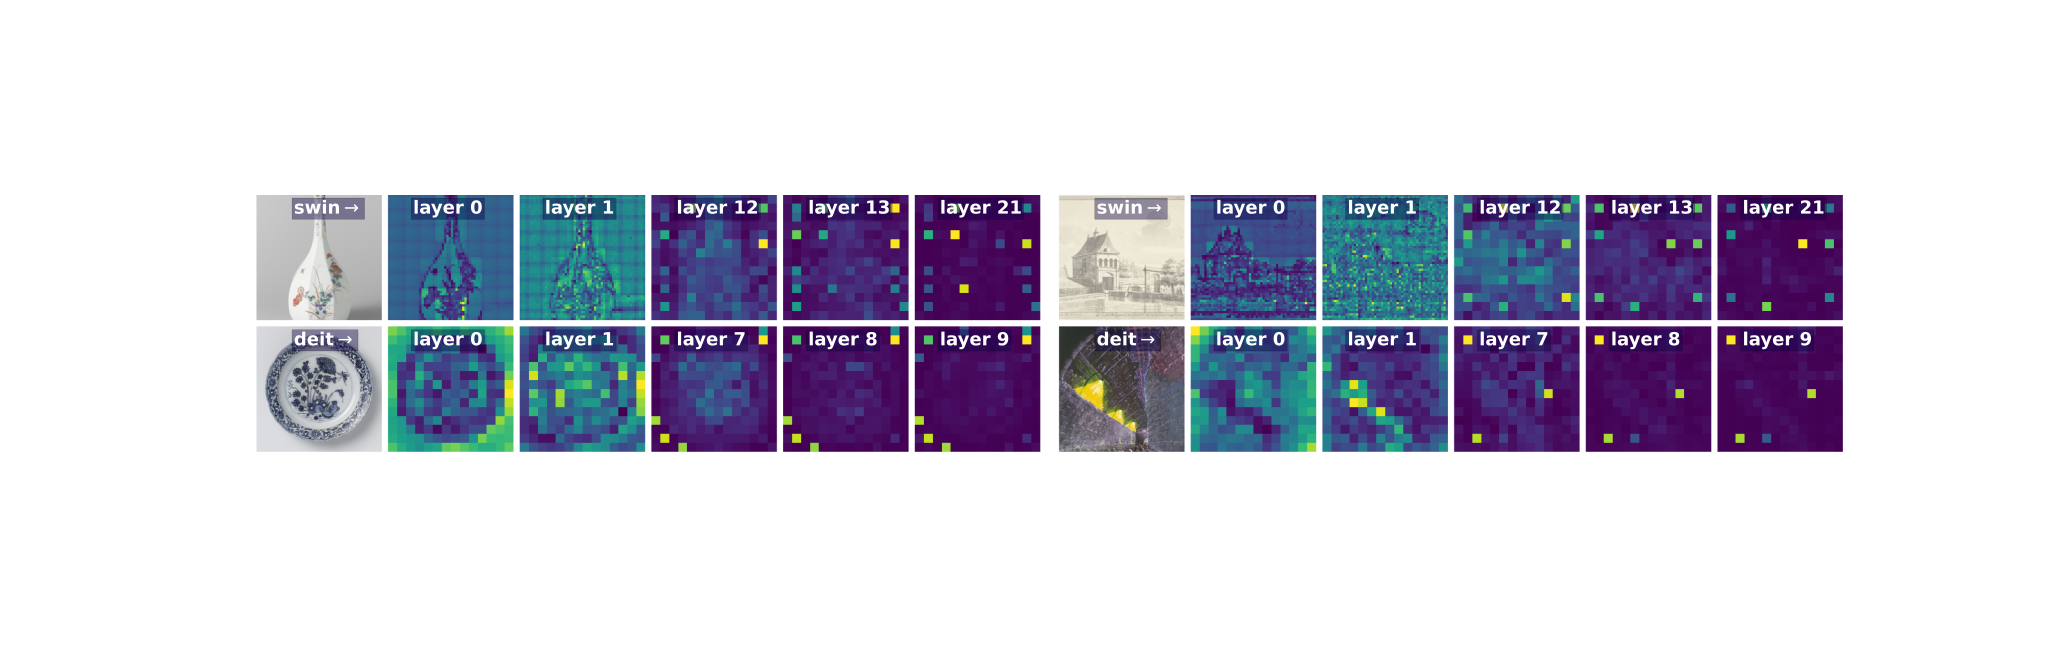
\includegraphics[width=\textwidth]{img/layers.png}

\centering
{\tiny \textbf{Saliency maps}}\\

\vspace{-0.3cm}
\begin{columns}
\column{0.5\textwidth}
\includegraphics[width=\textwidth]{img/img011_salience.png}
\column{0.5\textwidth}
\includegraphics[width=\textwidth]{img/img005_salience.png}
\end{columns}
\end{frame}
%-------------------------------------------------------------------------------


%-------------------------------------------------------------------------------
{
\setbeamercolor*{frametitle}{bg=white}
\begin{frame}
\centering
\textsc{\Huge \textbf{That's} all!}

\pause
{\small except for the questions :-)}
\end{frame}
}
%-------------------------------------------------------------------------------

%-------------------------------------------------------------------------------
\begin{frame}[t, allowframebreaks]
\createtitle{References}
\bibliographystyle{acm}
{\tiny
\bibliography{literature}}
\end{frame}
%-------------------------------------------------------------------------------

\end{document}
